\documentclass[a4paper,12pt]{article}
\usepackage[utf8]{vietnam}
\usepackage{amsmath}
\usepackage{graphicx}

\title{Phân tích rủi ro khi đánh tài xỉu theo phương pháp gấp thếp}
\author{Dương Văn Giỏi}
\date{}

\begin{document}

\maketitle

\begin{center}
    Trường Công nghệ Thông tin - Đại học Bách Khoa Hà Nội \\
    10 Tạ Quang Bửu, Bách Khoa, Hai Bà Trưng, Hà Nội, Việt Nam \\
    E-mail: gioi.trongxuan@gmail.com / gioi.dv215041@sis.hust.edu.vn
\end{center}

\begin{abstract}
    Phương pháp gấp thếp là một chiến lược phổ biến trong cá cược tài xỉu, trong đó người chơi sẽ nhân đôi số tiền cược sau mỗi lần thua để đảm bảo có lãi khi thắng. Tuy nhiên, vấn đề phát sinh khi gặp 'cầu bệt' - một chuỗi liên tiếp cùng kết quả kéo dài, có thể dẫn đến thua lỗ nhanh chóng. Bài báo này phân tích xác suất xuất hiện cầu bệt, giới hạn của phương pháp gấp thếp và điều kiện để người chơi đạt lợi nhuận mong muốn với mức rủi ro thấp. Hiện tại bài toán chỉ đang tiếp cận dưới điều kiện tiêu chuẩn, giả thuyết thuận lợi. Tương lai sẽ phát triển và thêm nhiều tham số hơn. Mọi dữ liệu trong bài viết đều là giả định, không thực tế.
\end{abstract}

\tableofcontents

\section{Giới thiệu}
Trong trò chơi tài xỉu, nhiều người chơi sử dụng phương pháp gấp thếp, tức là sau mỗi lần thua, họ nhân đôi tiền cược với hy vọng gỡ lại toàn bộ số tiền đã mất và có lãi khi thắng. Tuy nhiên, phương pháp này gặp một vấn đề lớn khi xuất hiện "cầu bệt" – tức là chuỗi tài hoặc xỉu liên tục kéo dài. Bài viết này sẽ phân tích xác suất xuất hiện cầu bệt, giới hạn của phương pháp gấp thếp, và điều kiện để người chơi có thể đạt được lợi nhuận mong muốn với mức rủi ro chấp nhận được.

\begin{figure}[h]
    \centering
    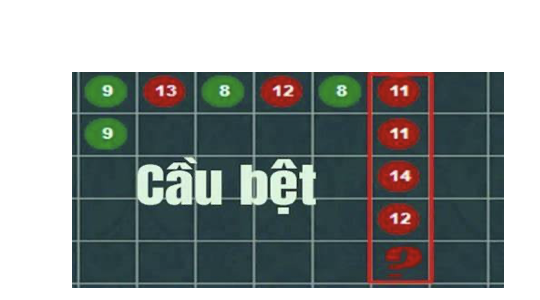
\includegraphics[width=0.5\textwidth]{cau_bet.png}
    \caption{Cầu bệt là gì?}
\end{figure}

\section{Mô hình toán học}

\subsection{Tổng tiền cược}
Giả sử tiền cược ban đầu là $a$, tổng vốn là $A$, khi áp dụng chiến lược gấp thếp, tổng tiền cược sau $n$ lần cược có thể tính bằng công thức:
\[
\text{Tổng tiền cược} = a + 2a + 4a + \ldots + 2^n \cdot a
\]
Đây là tổng của một cấp số nhân có công thức tổng quát:
\[
S_n = (2^n - 1) \cdot a
\]
Số lần cược tối đa có thể thực hiện trước khi hết vốn là:
\[
n = \log_2 \left(\frac{A}{a} + 1\right)
\]

\begin{figure}[h]
    \centering
    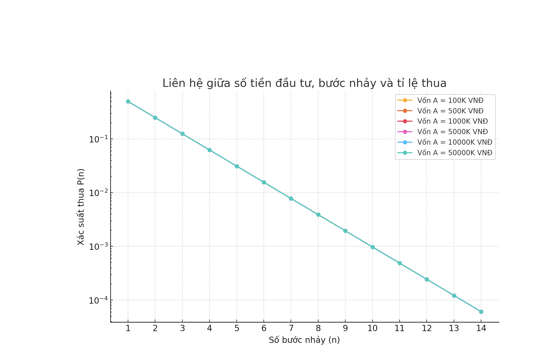
\includegraphics[width=0.5\textwidth]{xac_suat_thua.png}
    \caption{Xác suất thua bước nhảy}
\end{figure}

\subsection{Xác suất cầu bệt}
Nếu xác suất xuất hiện tài hoặc xỉu là 50\%, thì xác suất cầu bệt kéo dài $k$ lần là:
\[
P(k) = (0.5)^k
\]
Thực tế, cầu bệt thường có thể kéo dài từ 8 đến 9 lần, gây rủi ro lớn cho người chơi sử dụng chiến thuật gấp thếp.

\begin{figure}[h]
    \centering
    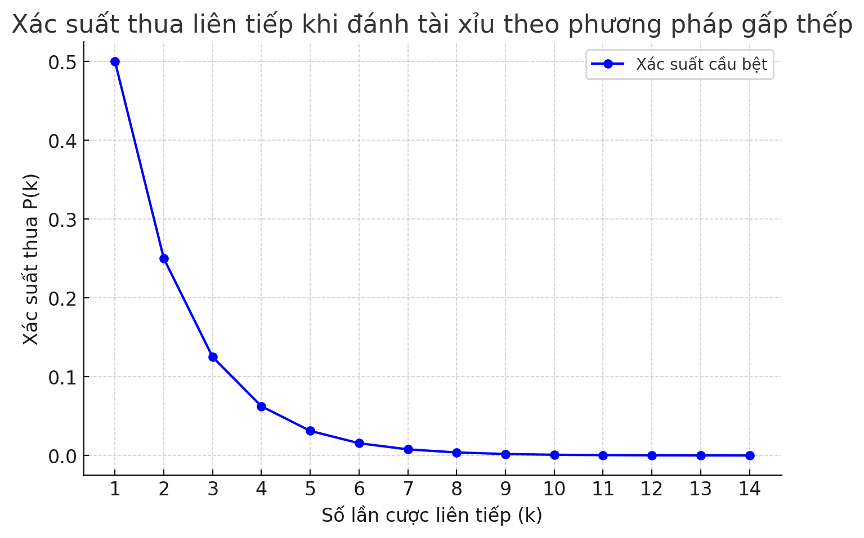
\includegraphics[width=0.5\textwidth]{xac_suat.png}
    \caption{Xác suất Bệt}
\end{figure}

\section{Bài toán thực tế}
Giả sử Nam có tổng vốn $A = 1$ triệu VND, Nam muốn xác định mức cược tối thiểu $a$ để đảm bảo có thể thu về 1.5 triệu VND với rủi ro $<$ 1\%.
\subsection{Điều kiện số lần cược tối đa}
Để rủi ro $<$ 1\%, ta giả sử Nam cần có đủ vốn để chịu được ít nhất $n = 7$ lần cược liên tiếp thua.
\[
\log_2\left(\frac{1000}{a} + 1\right) \geq 7
\]
Giải bất phương trình:
\[
\frac{1000}{a} + 1 \geq 128
\]
\[
\frac{1000}{a} \geq 127
\]
\[
a \leq 7.87 \text{ (VND)}
\]
Vậy mức cược tối thiểu mà Nam có thể đặt để đảm bảo tồn tại đủ lâu trong trò chơi là 7.87 nghìn VND.

\subsection{Số chu kỳ thắng cần thiết}
Nam muốn thu về 1.5 triệu VND, nghĩa là lợi nhuận cần đạt là 500 nghìn VND. Số chu kỳ thắng cần đạt được là:
\[
W \geq \frac{500}{a} = \frac{500}{7.87} \approx 64 \text{ (chu kỳ)}
\]

\subsection{Thời gian cần thiết}
Mỗi lượt chơi tài xỉu bao gồm 50 giây cược + 10 giây xem kết quả (tổng cộng 1 phút mỗi lượt).

\begin{figure}[h]
    \centering
    
\includegraphics[width=0.5\textwidth]{giaodien.png}
    \caption{Giao diện tài xỉu}
\end{figure}

Giả sử trung bình mỗi chu kỳ thắng kéo dài 4 lượt chơi, thì tổng thời gian cần thiết để đạt được 64 chu kỳ thắng là:
\[
T \geq 64 \times 4 = 256 \text{ phút} \approx 4.5 \text{ giờ}
\]
\section{Kiểm thử}
Với vốn ban đầu là 50,000 VND, ta thực hiện kiểm thử trên hệ thống Red88 với bước nhảy 1,000 VND. Kết quả như sau:

\begin{table}[h!]
    \centering
    \resizebox{\textwidth}{!}{%
    \begin{tabular}{|c|c|c|c|c|c|}
        \hline
        Số chu kỳ & Tiền cược (VND) & Xác suất thắng & Xác suất thua & Tỉ lệ thua tích thắng \\ \hline
        1 & 1,000 & 0.5 & 0.5 &  0.96875 \\ \hline
        2 & 3,000 & 0.75 & 0.25 &  0.9384765625 \\ \hline
        3 & 7,000 & 0.875 & 0.125 & 0.8265522132 \\ \hline
        4 & 15,000 & 0.9375 & 0.0625 &  0.46674661 \\ \hline
        5 & 31,000 & 0.96875 & 0.03125 & 0.02215163882 \\ \hline
        6 & 63,000 & 0.984375 & 0.015625 & 0.0000000001181503929 \\ \hline
        7 & 127,000 & 0.9921875 & 0.0078125 &  0 \\ \hline
        8 & 255,000 & 0.99609375 & 0.00390625 &  0 \\ \hline
        9 & 511,000 & 0.998046875 & 0.001953125 & 0 \\ \hline
        10 & 1,023,000 & 0.9990234375 & 0.0009765625 & 0 \\ \hline
        11 & 2,047,000 & 0.9995117188 & 0.00048828125 &  - \\ \hline
    \end{tabular}%
    }
    \caption{Kết quả kiểm thử với vốn ban đầu 50,000 VND và bước nhảy 1,000 VND}
\end{table}
\begin{figure}[h]
    \centering
    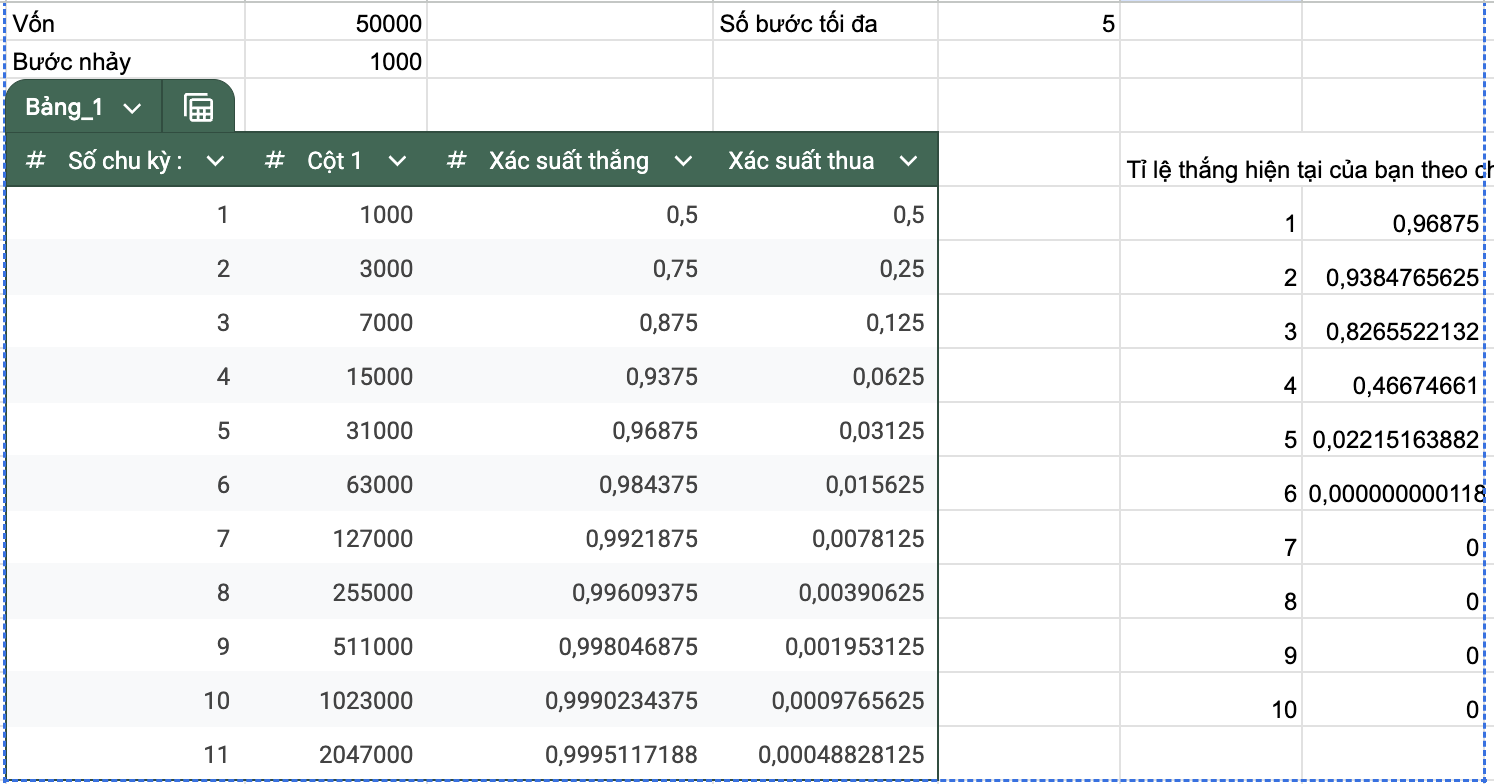
\includegraphics[width=0.5\textwidth]{losss.png}
    \caption{Biểu đồ minh họa tổn thất}
\end{figure}
Kết quả phân tích cho thấy, với vốn khởi điểm 50,000 VND và mức cược tăng dần theo bước nhảy 1,000 VND, người chơi chỉ có thể duy trì tối đa 5 lần cược trước khi cạn vốn. Tỷ lệ thắng tích lũy giảm dần theo số chu kỳ, trong khi rủi ro thua lỗ tăng lên nhanh chóng khi đối mặt với chuỗi cầu bệt kéo dài. Điều này nhấn mạnh rằng việc quản lý vốn và hiểu rõ giới hạn của chiến lược gấp thếp là yếu tố then chốt để giảm thiểu rủi ro trong trò chơi.
Vấn đề tiếp theo là vấn đề rủi ro tích lũy, tức là tỉ lệ thua tích lũy sẽ tăng dần theo số chu kỳ. Điều này có nghĩa là người chơi sẽ mất toàn bộ vốn . Giả sử tỷ lệ thắng mỗi chu kỳ là 99\% sau khi thắng liên tục 10 chu kỳ, tỷ lệ thắng lúc đó là : $0.99^{10} = 0.9043820750088049$.  Nhưng để đạt được mức tỉ lệ thắng 99\% người chơi chỉ có thể đánh tỉ lệ vốn / mức ăn là > 127 lần. Giả dụ bạn đánh 10000/ lần thì vốn phải là 1tr270k và tỉ lệ lãi được 100K là  90\%.
Nếu bạn đánh tỷ lệ thắng 90\% 1 lần thì tỷ lệ thắng 10 lần chỉ còn 34\%. 
\section{Kết luận}
Với vốn ban đầu 1 triệu VND, Nam cần đặt mức cược tối thiểu 7.87 nghìn VND để duy trì khả năng gỡ vốn trong trường hợp gặp cầu bệt dài. Đồng thời, để đạt được lợi nhuận 500 nghìn VND, Nam cần trải qua 64 chu kỳ thắng, tương đương với 4.5 giờ chơi liên tục. Tuy nhiên, cần lưu ý rằng chiến thuật gấp thếp luôn có rủi ro cao, và nếu cầu bệt kéo dài hơn dự kiến, người chơi có thể mất toàn bộ vốn.
\end{document}
